\documentclass{beamer}

\mode<presentation>

\usetheme{Frankfurt}%
\usecolortheme{seagull}
\usepackage{multimedia}
%\usepackage{movie15}

\logo{
\includegraphics[height=.25in]{clarksonGreen}}

%\definecolor{garnet}{RGB}{179,0,91}
%\definecolor{garnet}{RGB}{108,43,53}
\definecolor{garnet}{RGB}{136,0,0}
%\definecolor{clarksonGreen}{RGB}{0,71,28}
\definecolor{clarksonGreen}{RGB}{0,52,21}
\setbeamercolor{palette primary}{fg=clarksonGreen,bg=white}
\setbeamercolor{palette secondary}{fg=clarksonGreen,bg=white}
\setbeamercolor{palette tertiary}{fg=clarksonGreen,bg=white}
\setbeamercolor{palette quaternary}{bg=clarksonGreen,fg=white}
\setbeamercolor{block title}{fg=black,bg=black!15}
\setbeamercolor{block body}{fg=black,bg=black!10}
\setbeamercolor{titlelike}{bg=clarksonGreen,fg=white} % parent=palette quaternary}



% Misc definitions that are nice to have
\newcommand{\lp}{\left(}
\newcommand{\rp}{\right)}



%\usepackage{pgfpages}
%%\pgfpagesuselayout{resize}[border shrink=5mm,landscape]
%\pgfpagesuselayout{2 on 1}[border shrink=5mm]



\begin{document}

\title{Mission Model}
\subtitle{Software Development}
\author{MADC Team}
\institute{Clarkson University}
%\date{8 July 2009}
\date{14 June 2011}

\begin{frame}
  \titlepage
  \begin{abstract}
    Broad overview of the software development of the mission
    model. The mission model is implemented in python with each agent
    represented by a separate class. Underlying supporting classes
    encapsulate the way information is exchanged and interpreted.
  \end{abstract}
\end{frame}



\begin{frame}
  \frametitle{Schedule}

  \begin{itemize}
  \item Software Development (This discussion) 
  \item Network Implementation - Design Considerations
  \item Lunch
  \item Core Demonstration
  \end{itemize}

\end{frame}


\begin{frame}
  \frametitle{Outline}
  \tableofcontents[pausesection,hideallsubsections]
\end{frame}



\section{Conceptual Model}


\begin{frame}
  \frametitle{Conceptual Model}

  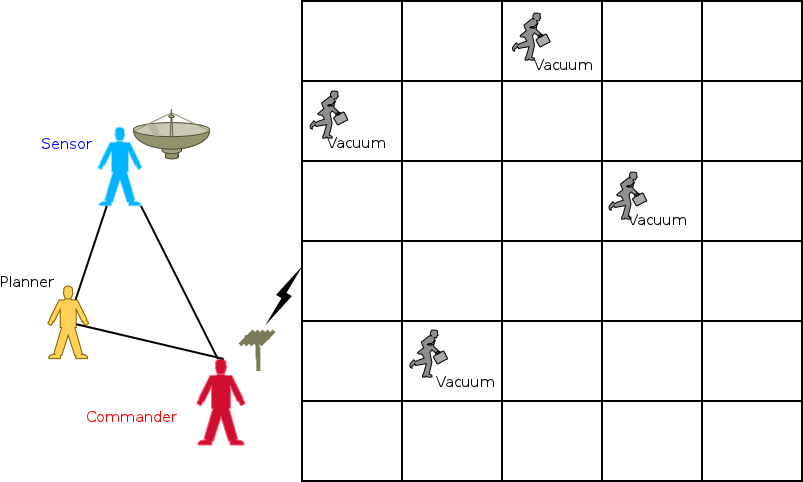
\includegraphics[height=6cm]{conceptualWorld.png}

\end{frame}


\begin{frame}
  \frametitle{Computational Model}
  \only<1>{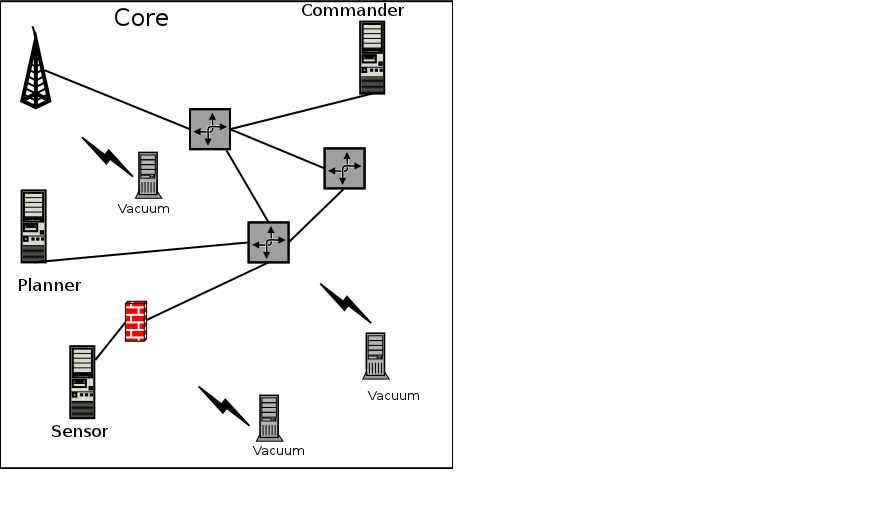
\includegraphics[height=6cm]{computationalMissionCore.png}}
  \only<2>{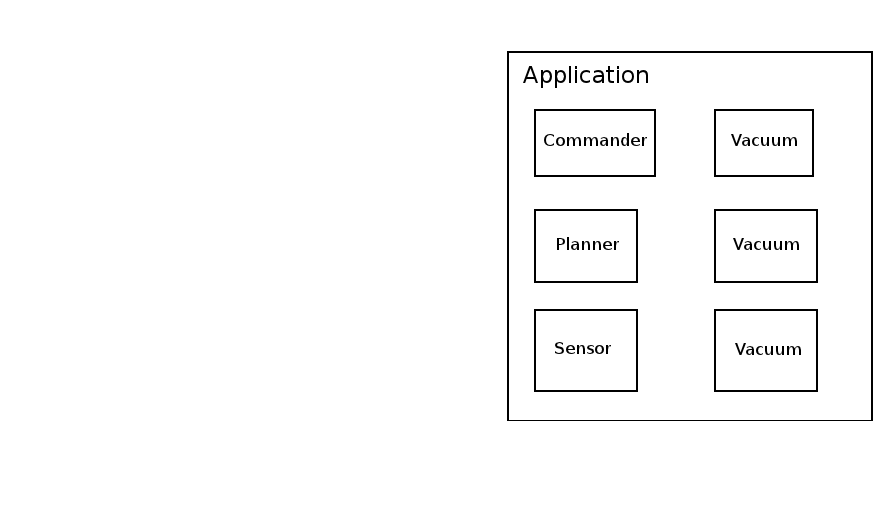
\includegraphics[height=6cm]{computationalMissionPython.png}}
  \only<3>{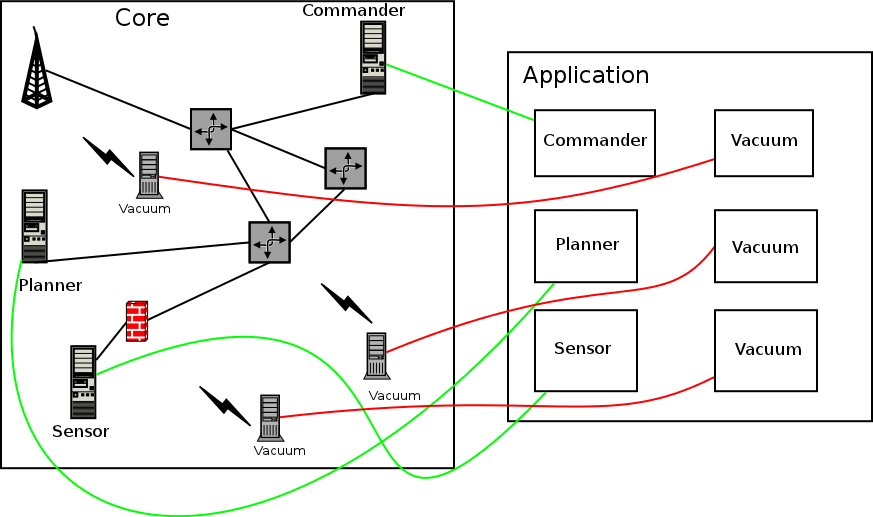
\includegraphics[height=6cm]{computationalMission.png}}
\end{frame}


\begin{frame}
  \frametitle{Why}

  {In a nutshell:}

  \begin{itemize}
  \item<1-> This is the subject of Todd and Pat's discussion which
    will follow.
  \item<2-> We need flexible implementation.
  \item<2-> We need flexible configurations and data management.
  \end{itemize}
  

\end{frame}


\section{Simulation Requirements}

\begin{frame}
  \frametitle{Simulation Requirements}

  \begin{itemize}
  \item Want to run multiple instances of a simulation. (Parallel
    model evaluation.)
  \item Need to get data quickly and easily.
  \item Need to make changes during execution:
    \begin{itemize}
    \item Change a parameter set.
    \item Stop a simulation
    \item Start a simulation.
    \item Query the state of a simulation via an external request.
    \end{itemize}
  \end{itemize}

\end{frame}


\begin{frame}
  \frametitle{Application Goals}

  \begin{itemize}
  \item Agents need to communicate with each other.
  \item Communication interface should be through standard network
    API's (ex: library calls through Python TCP classes.)
  \item Access to data with minimal impact to the simulation but do it
    in a distributed environment.
  \item Make changes to the simulation while it is running.
  \item Implement the mission model on a wide range of computational
    platforms.
  \end{itemize}


\end{frame}

\begin{frame}
  \frametitle{Network Goals}

  \begin{itemize}
  \item Allow flexibility for a wide range of networks.
  \item Be able to monitor the network in a way that is consistent
    with ``real'' network monitoring tools.
  \item Be able to configure the network with minimal \textit{a
      priori} knowledge of the application.
  \item Be able to exchange data in a seamless fashion with minimal
    impact to the simulation.
  \end{itemize}

\end{frame}


\section{Implementation Details}

\begin{frame}
  \frametitle{Core}

  Todd and Pat will discuss this.

\end{frame}


\begin{frame}
  \frametitle{Encapsulating Agent Communications}

  Each agent has a mission and a communication channel:

  \only<1>{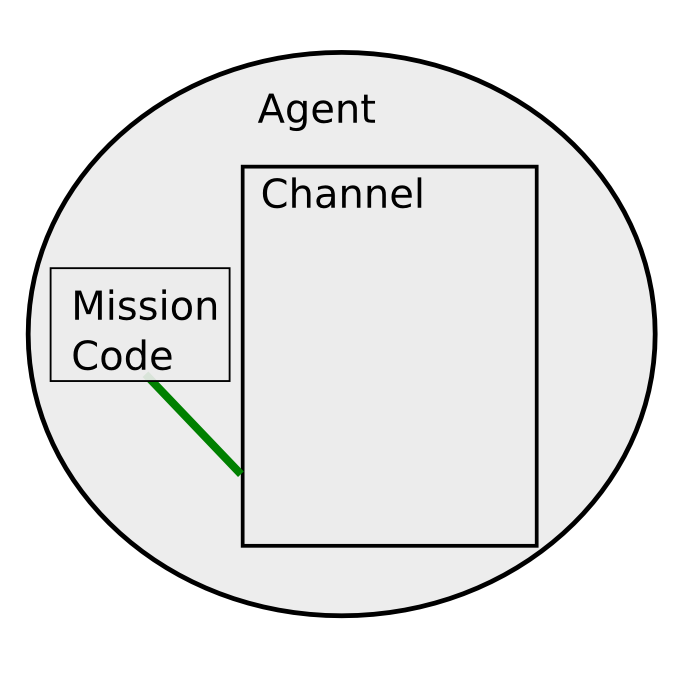
\includegraphics[height=7.0cm]{agent}}
  \only<2>{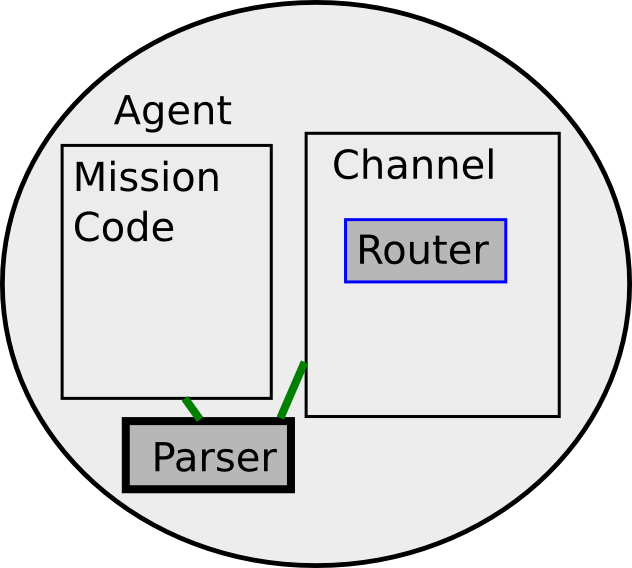
\includegraphics[height=7.0cm]{agentRouter}}
  \only<3>{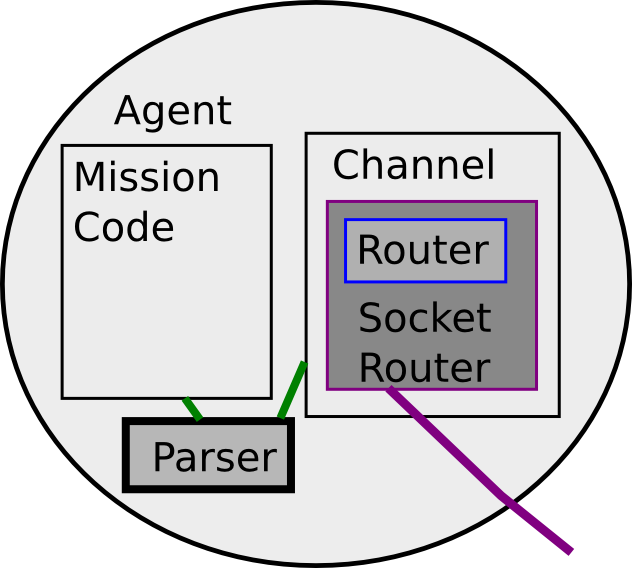
\includegraphics[height=7.0cm]{agentSocketRouter}}

\end{frame}


\begin{frame}
  \frametitle{Data Exchange Considerations}

  \begin{itemize}
  \item Data exchange occurs over network.
  \item Data exchange between agents within simulation should be
    consistent with external requests.
  \item Want portable parser using industry standard formats.
  \item Have investigated numerous approaches:
    \begin{itemize}
    \item HAL
    \item GME
    \item OWL
    \end{itemize}
  \item Currently using XML format based heavily on HAL-DIF.
  \item OWL appears to offer the best alternative.
  \end{itemize}
  

\end{frame}




%\begin{frame}
%  \frametitle{Test Cases}
%
%  $r=2$, $\alpha=0.5$.
%
%  \begin{columns}[t]
%    \column{.5\textwidth}
%    \centerline{\includegraphics[height=5.0cm]{meanError-r2-alpha0_5}}
%
%    \column{.5\textwidth}
%    \centerline{\includegraphics[height=5.0cm]{varError-r2-alpha0_5}}
%  \end{columns}
%
%\end{frame}



%  \begin{columns}[t]
%    
%    \column{.5\textwidth}
%    \begin{block}{Barney?}
%      Is it okay to trust your kids with Barney?
%    \end{block}
%    \pause
%  
%    \column{.5\textwidth}
%    \begin{block}{No, not Barney!}
%      Probably not.
%    \end{block}
%
%  \end{columns}
%
%
%\end{frame}





\begin{frame}
  \frametitle{}

  \centerline{\textbf{\Large Questions?}}
  
\end{frame}



\end{document}

% LocalWords:  Clarkson pausesection hideallsubsections
